\chapter{Preliminary analysis}

\section*{Introduction}

\hspace*{0.777cm} The first chapter of this report aims to provide an overview of the host and the client companies,
present the case study by highlighting the problem to be addressed and introduce the modeling language
used for the project. This chapter sets the stage for the subsequent sections by establishing the
context, significance and scope of the actions undertaken in the next chapters.

%=============================================================
\section{\fontsize{15}{18}\selectfont Presentation of the enterprises}
%=============================================================

\subsection{\fontsize{14}{17}\selectfont Technique Solution Et Innovation Industriel (TS2I)}
%-------------------------------------------------------------

\hspace*{0.777cm} TS2I is a leading company in the field of specialised machines fabrication, automation, industrial
maintenance, and Tampographique service. With a strong commitment to quality, innovation and
customer satisfaction, TS2I has established itself as a trusted partner for various industries.
The following provides an overview of TS2I and highlights its expertise in fabrication machines,
automation, industrial maintenance and pad printing services.

\begin{itemize}

    \item \textbf{Fabrication of specialised machines:} TS2I specializes in the design, development
    and production of specialised machines. These machines are tailored to meet the
    unique requirements of clients in diverse industries such as automotive, aerospace, electronics,
    and more. With a team of experienced engineers and technicians, TS2I leverages cutting-edge
    technologies to deliver custom fabrication machines that optimize productivity, efficiency and
    quality. Whether it's automated assembly lines, robotic systems or specialized machining
    equipment, TS2I ensures that each machine is built to the highest standards.

    \item \textbf{Automation:} Automation plays a crucial role in enhancing productivity and reducing
    operational costs. TS2I offers comprehensive automation solutions to help businesses automate
    their processes. From simple control systems to complex integrated automation solutions, TS2I
    designs and implements tailored solutions based on clients requirements. Their
    expertise in PLC programming, HMI design, robotics and motion control allows them to deliver
    efficient and reliable automation solutions that streamline operations and improve overall
    efficiency.

    \item \textbf{Industrial maintenance:} TS2I understands the importance of maintaining industrial
    equipment to ensure optimal performance and minimize downtime. The company offers comprehensive
    maintenance services to address the unique needs of its clients. Whether it's preventive
    maintenance, troubleshooting or equipment repair, TS2I's skilled technicians and engineers are
    well-equipped to handle a wide range of industrial machinery. By providing regular maintenance,
    TS2I helps clients avoid costly breakdowns, increase equipment lifespan and maximize
    productivity.

    \item \textbf{Tampographique service:} In addition to its fabrication machines and automation
    expertise, TS2I also offers a specialized service in tampography or pad printing. Tampography
    is a versatile printing technique used for applying designs or logos onto various surfaces
    including plastics, metals, ceramics and glass. TS2I's pad printing service ensures
    high-quality and precise printing, providing clients with branding solutions that are durable
    and visually appealing. Whether it's product customization, promotional items or industrial
    labeling, TS2I's pad printing service offers reliable and efficient solutions.

\end{itemize}

%-------------------------------------------------------------
\subsection{\fontsize{14}{17}\selectfont TESCA}
%-------------------------------------------------------------

\subsubsection{\fontsize{13}{16}\selectfont Presentation of the company}

\hspace*{0.777cm} Tesca Group is a family-run company with a background in textiles that has successfully ventured
into the automotive industry, specifically automotive seating. Emulating the approach of a French
automotive manufacturing house, Tesca Group meticulously crafts each piece, from its atelier to its
global production sites\cite{tesca_official}. The company strives to embody the same creative audacity and
prides itself on being a partner to major automotive manufacturers like:

\begin{figure}[H]
    \centering
    
\includegraphics[width=0.8\textwidth, keepaspectratio]{images/partners.png}
    \caption{Tesca's partners}
    \label{fig:chapter1-1}
\end{figure}

\hspace*{0.25cm}With a clientele consisting of demanding visionaries who shape the future of mobility, Tesca Group
positions itself as a reliable and flexible partner, accompanying its clients in their pursuit of
innovation and competitiveness. The company believes that adopting a long-term and eco-friendly
vision is crucial for sustainable growth, constantly pushing for excellence rather than settling for
mediocrity\cite{tesca_official}.


\begin{itemize}

    \item \textbf{Sustainability:} A concrete and integral part of Tesca Group's approach. The company is committed to sustainable development and actively incorporates environmental and social values into its products, services, and activities within the automotive industry. Since 2004, Tesca Group has been dedicated to controlling its ecological footprint, and the executive management maintains and expands upon these efforts. The company adheres to the values and principles of the Global Compact through its Ethics Charter, to obtain ISO~14001 certification for all its sites\cite{tesca_official}.

\end{itemize}



\begin{itemize}

    \item \textbf{Environmental policy:} Tesca Group's environmental policy revolves around five major directions: behaving in an environmentally responsible manner, controlling the industrial waste, optimizing energy consumption and natural resources, participating in the reduction of the ecological footprint throughout the design and production processes and ensuring compliance with environmental regulations and requirements\cite{tesca_official}.

\end{itemize}


\begin{itemize}

    \item \textbf{Innovation:} A driving force within Tesca Group, with a constant emphasis on generating new ideas and executing them effectively. The company's research programs focus on key themes in the automotive industry, such as weight reduction, optimized part design and ecological footprint expertise. While prioritizing user comfort, functionality and safety. Tesca Group holds numerous patents in the conception, design and manufacturing of automotive parts and seat components, including headrests, armrests, upholstery, padding and ``smart textiles''\cite{tesca_official}.

\end{itemize}


\begin{itemize}

    \item \textbf{Industrial excellence:} A cornerstone of Tesca Group's strategy, whether through its local production sites or research centers. The company strives to provide reliable processes that meet the evolving market expectations worldwide. Tesca Group empowers its teams through a culture of continuous improvement, with competitiveness, efficiency and exceptional service forming the foundation of its industrial success. SPRINT (Tesca's Industrial Production System) is employed to engage collaborators at all levels, aiming to standardize procedures and ensure perpetual progress in industrial performance. Shared values among Tesca Group employees include excellence, self-discipline, commitment, autonomy and pragmatism\cite{tesca_official}.

\end{itemize}


\begin{itemize}

    \item \textbf{Quality:} Tesca Group's Quality policy aligns with five major directions: meeting commitments to conformity, cost and deadlines; aligning industrial and purchasing performance with the highest quality criteria; standardizing existing processes to offer innovative products; prioritizing process control and prevention; and continuously enhancing the skills of its teams\cite{tesca_official}.

\end{itemize}



\begin{itemize}

    \item \textbf{History:} In terms of its history, Tesca Group has a notable timeline of achievements. Starting in 1960 with the provision of Citro\"en 2CV roofs, the company went on to pioneer and apply the Foam In Place technology in 1978. In 1983, Tesca Group established its Design Studio in Paris, followed by the creation of the CERA research and development center in Reims in 1993. By the year 2000, the company had expanded its production capabilities worldwide. In 2016, Tesca Group underwent a significant transformation, becoming Tr\`eves TSC\cite{tesca_official}.

\end{itemize}



\hspace*{0.25cm}Overall, Tesca Group has established itself as a reputable partner to major automotive manufacturers
driven by a commitment to sustainability, innovation, industrial excellence and quality. Through its
diverse range of products and services, the company aims to shape the future\cite{tesca_official}.

\subsubsection{\fontsize{13}{16}\selectfont Technical file}

The following table presents the technical file of TESCA.

\begin{table}[H]
    \centering
    \caption{Technical file of TESCA}
    \begin{tabular}{|l|l|}
        \hline
        \textbf{Company name} & \textbf{TESCA} \\
        \hline
        \textbf{Sector} & Vehicle interior equipment \\
        \hline
        \textbf{Creation} & 2019 \\
        \hline
        \textbf{Legal form} & Foreign company \\
        \hline
        \textbf{Staff} & 179 employees \\
        \hline
        \textbf{Address} & Grombalia Industrial Zone – Nabeul– Tunisia \\
        \hline
    \end{tabular}
\end{table}

\subsubsection{\fontsize{13}{16}\selectfont Organizational chart}

The organizational chart shown in Figure 2 presents the distribution of positions and functions within the Tesca enterprise.

\begin{figure}[H]
    \centering
    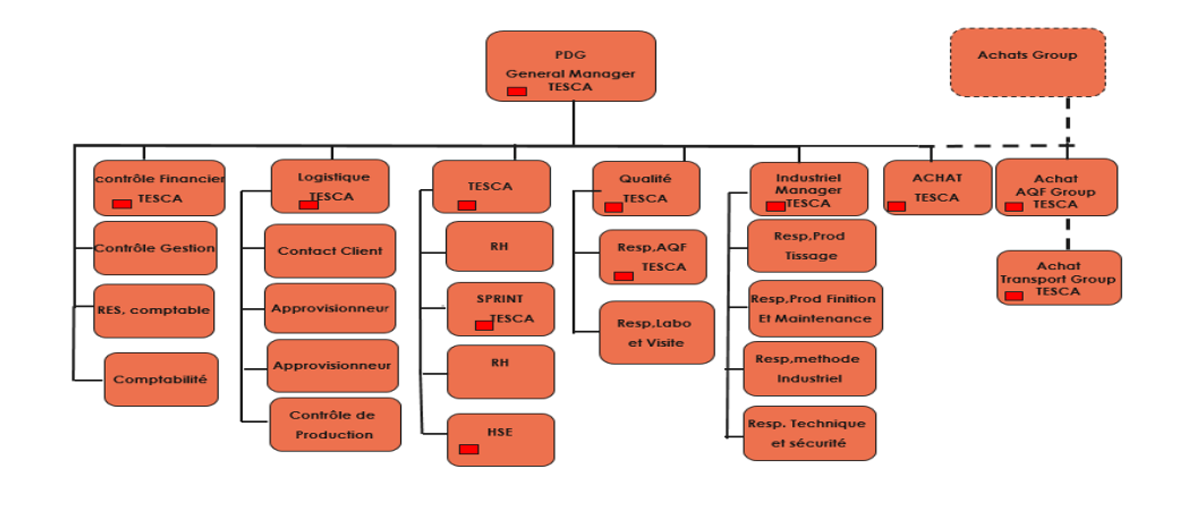
\includegraphics[width=0.95\textwidth, keepaspectratio]{images/organigramme.png}
    \caption{Organizational chart of TESCA}
    \label{fig:chapter1-2}
\end{figure}

\section{\fontsize{15}{18}\selectfont Case study}

\subsection{\fontsize{14}{17}\selectfont Overview of the Existing System}

\hspace*{\parindent} The existing production monitoring system was developed  to replace manual paper-based stop recording with automated digital tracking. The system consists of three components working together: a Delta DVP PLC installed on the fabric inspection machine, a Node-RED platform serving as the intermediary that reads PLC data and communicates with the database, and a MySQL database storing all production information.

Before this system existed, operators manually recorded all machine stops, causes, and durations on paper during their shifts. This process was prone to errors, made it hard to monitor, and could not conduct real-time analysis. In the new system, the PLC senses when the machine is stopped; the operator selects the reason for the stoppage via a tablet, and the system automatically computes the time the machine takes to start.

There are two main users of the system. Operators on the production floor use a tablet application that displays real-time machine speed, yardage measurements, lighting controls, and a dropdown menu to select stop causes. This interface updates continuously and provides immediate feedback, making it practical for shop-floor use. Managers access a web interface where they can filter data by date and shift team, view a table of all stops with their causes and durations, see a bar chart showing which causes are most frequent, and view the daily OEE (Overall Equipment Effectiveness) metric that measures productive time versus downtime.

\begin{figure}[H]
\centering
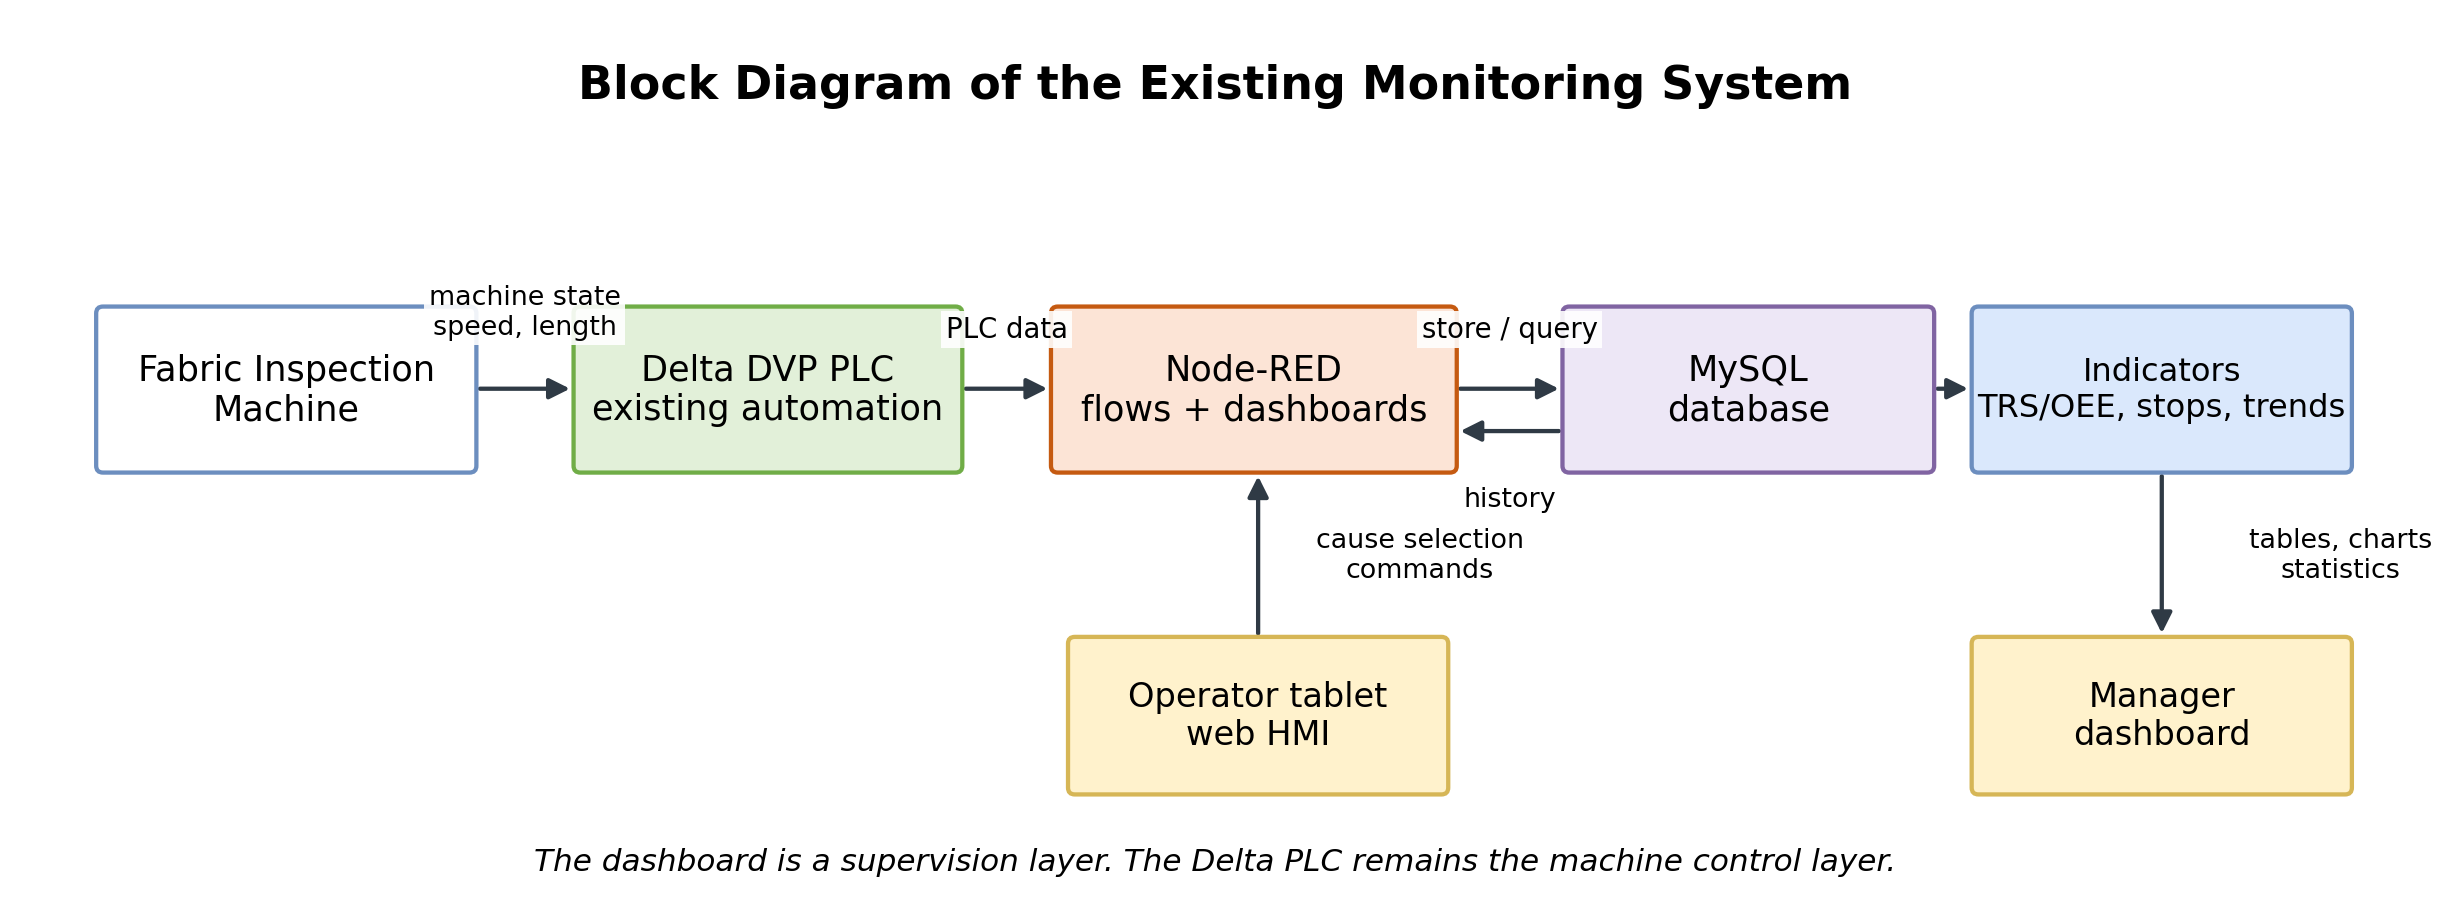
\includegraphics[width=0.9\textwidth, keepaspectratio]{images/block_diagram.png}
\caption{Block Diagram of the Production Monitoring System}
\label{fig:chapter1-3}
\end{figure}

\begin{figure}[H]
\centering
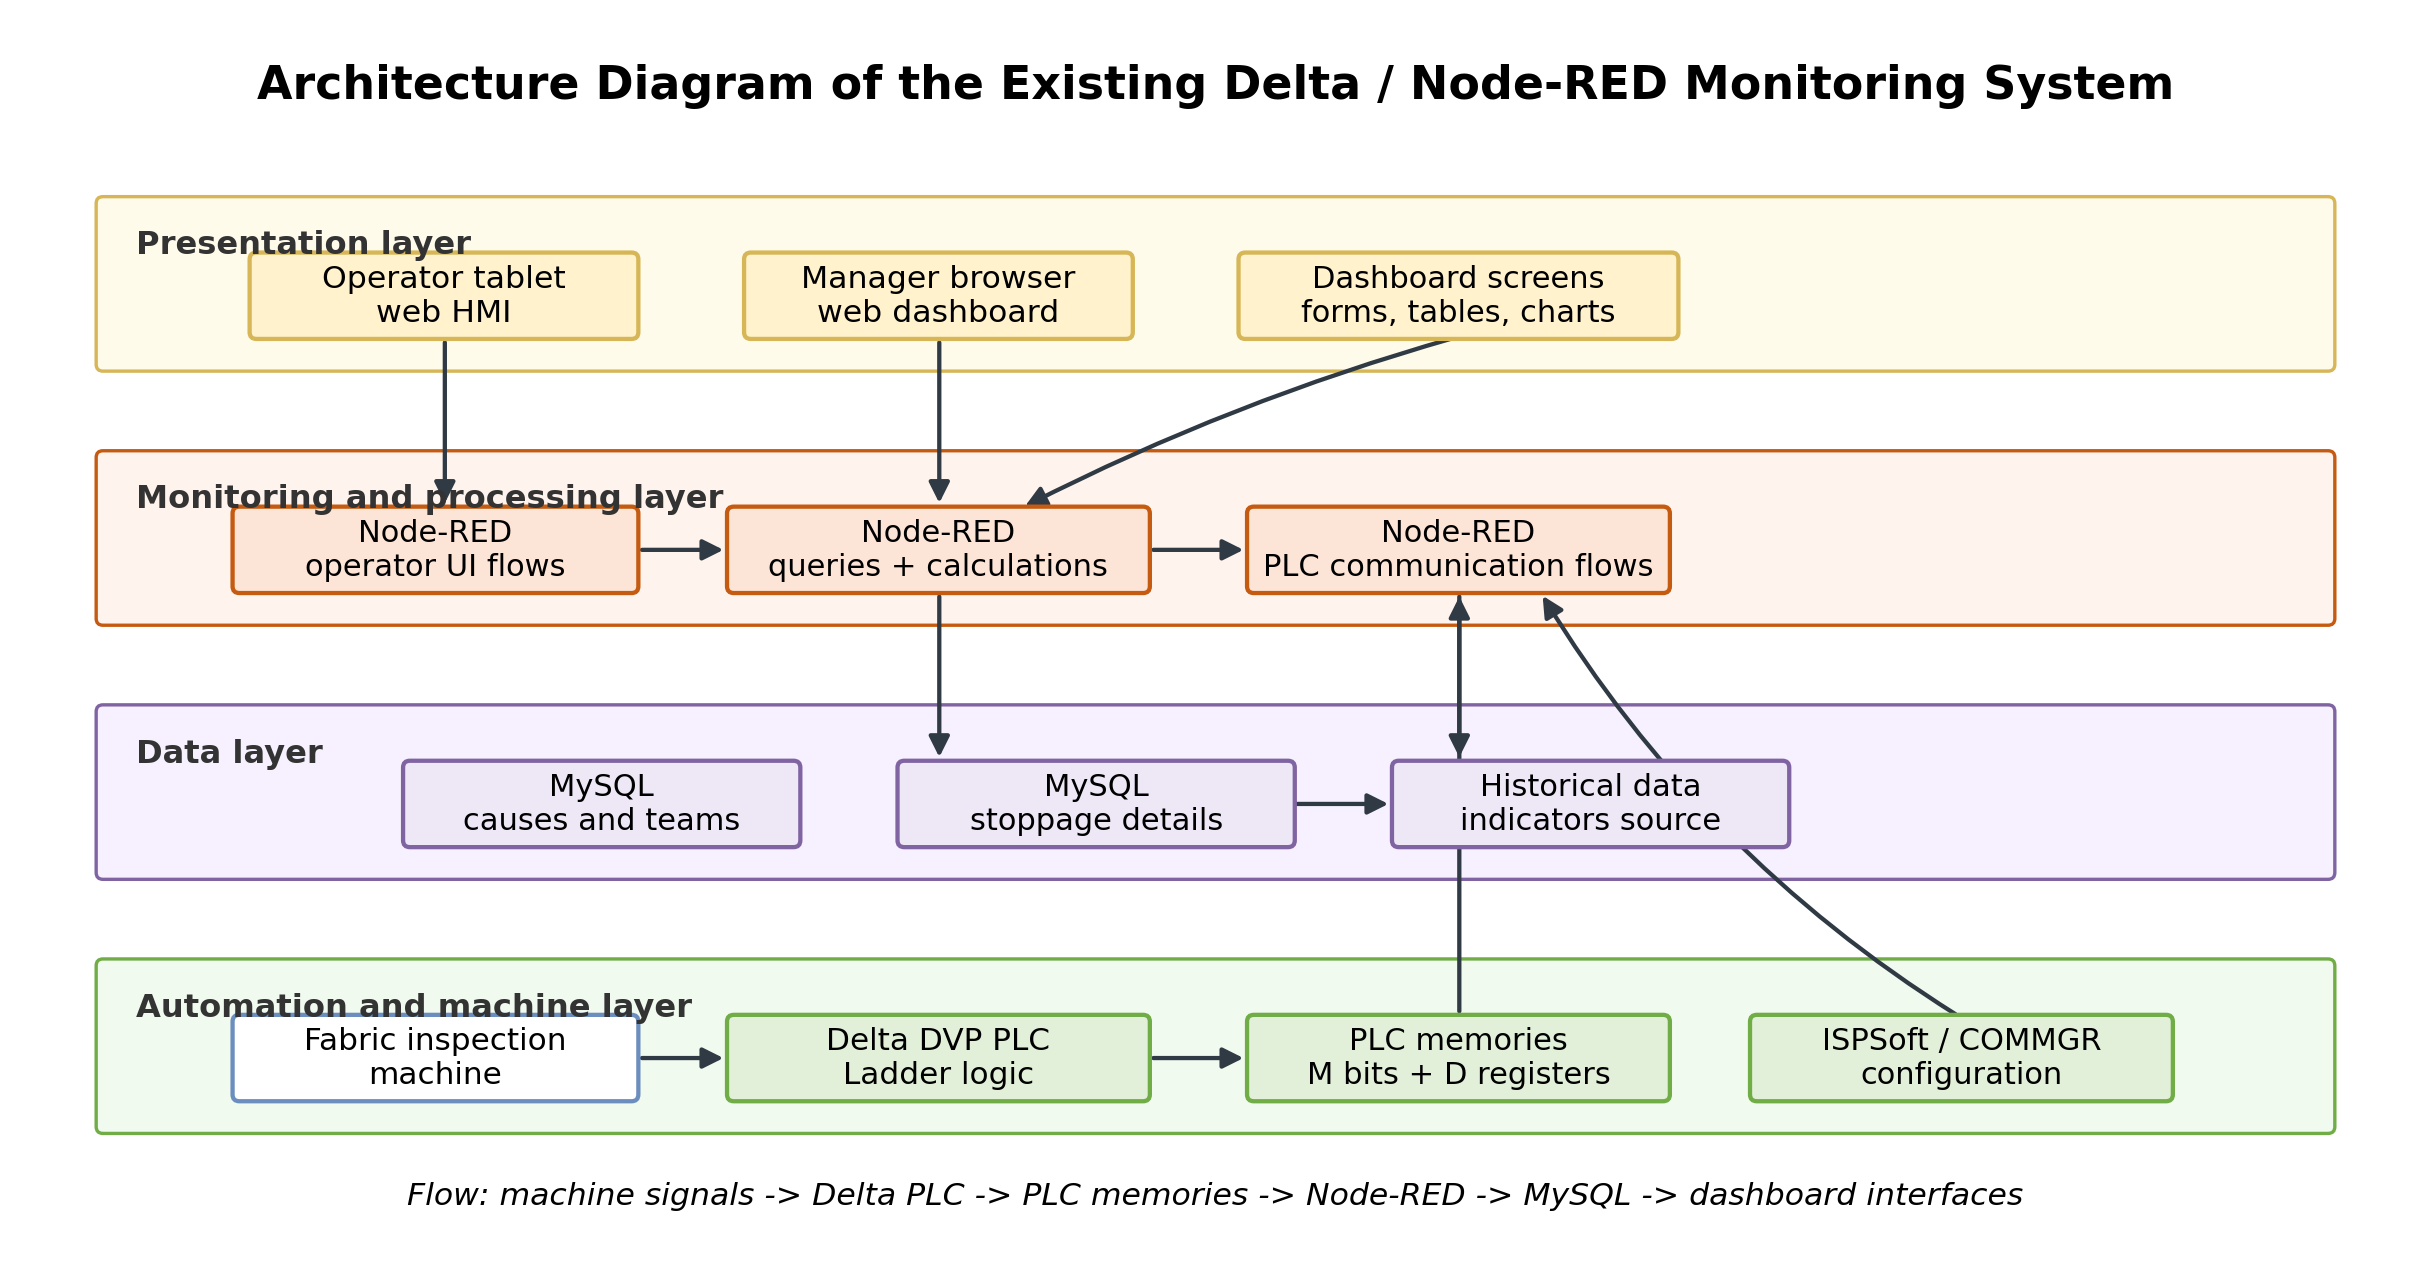
\includegraphics[width=0.9\textwidth, keepaspectratio]{images/architecture_diagram.png}
\caption{Architecture Diagram of the Production Monitoring System}
\label{fig:chapter1-4}
\end{figure}

\subsection{\fontsize{14}{17}\selectfont Criticism of the existing system}

\subsubsection{\fontsize{13}{16}\selectfont Limited Data Analysis}

\hspace*{\parindent} The existing system successfully records stops but provides limited analytical capability. The manager interface shows a bar chart of stop causes and a table of stops for the selected period, but it does not show trends over time. A manager viewing one week of data sees aggregated numbers but cannot easily see whether the situation is improving or deteriorating day by day. The interface does not enable comparison between teams or shifts, making it difficult to identify performance patterns.

\subsubsection{\fontsize{13}{16}\selectfont No Real-Time Manager Updates}

\hspace*{\parindent} A significant limitation is that the manager web interface does not automatically update. When a manager opens the dashboard to check production status, they must manually click a filter button to retrieve current data. If new stops occur after they view the data, these are not automatically displayed—the manager sees the situation as it was at their last manual refresh. In production environments, delays in visibility can mean slower response to problems.

\subsubsection{\fontsize{13}{16}\selectfont Limited Performance Metrics}

\hspace*{\parindent} The system primarily reports OEE and stop causes. Modern production monitoring typically tracks additional metrics to provide a complete picture. The system does not show trends in OEE over time, separate availability from performance metrics, or provide any predictive capability to identify potential problems before they occur. A manager cannot easily identify whether equipment health is improving or deteriorating, or whether specific causes show patterns that might indicate underlying issues.

\subsubsection{\fontsize{13}{16}\selectfont Inflexible User Interface and Limited Access}

\hspace*{\parindent} All managers see the same view regardless of their role or needs. The interface is designed for desktop computers and is not optimized for mobile devices, meaning managers cannot check production status from a smartphone while away from their office. There is also no concept of custom dashboards where different users might want different information.

\subsubsection{\fontsize{13}{16}\selectfont Data Quality and Verification}

\hspace*{\parindent} The system relies on operators to manually select stop causes from a dropdown menu. There is potential for human error or inconsistency in cause selection. Once a cause is recorded, there is no verification process or audit trail to show who entered the data or when. If a data discrepancy is discovered later, there is no way to trace back what happened.

\subsubsection{\fontsize{13}{16}\selectfont Lack of Security and Integration}

\hspace*{\parindent} The existing system has no user authentication or access control. Anyone with the IP address can access all production data without logging in. The system also cannot export data to other formats or systems. If a manager needs to perform advanced analysis in Excel or if another department needs production data, it must be manually copied or requested.

\subsubsection{\fontsize{13}{16}\selectfont Scalability Concerns}

\hspace*{\parindent} The Node-RED platform handles all functions in a monolithic design: reading from the PLC, storing in the database, and serving both the operator tablet and manager web interface. As data volume grows or additional machines are added, this architecture may face performance or reliability issues, since any slowdown in one function could impact others.

\subsection{\fontsize{14}{17}\selectfont Specifications Book}

\hspace*{\parindent} The system to be developed shall improve the existing monitoring dashboard by strengthening real-time supervision, data reliability, traceability, analysis capabilities and user access control. It shall continue to use the production data made available by the existing industrial environment and shall not disturb the machine control logic executed by the Delta PLC.

\begin{figure}[H]
\centering
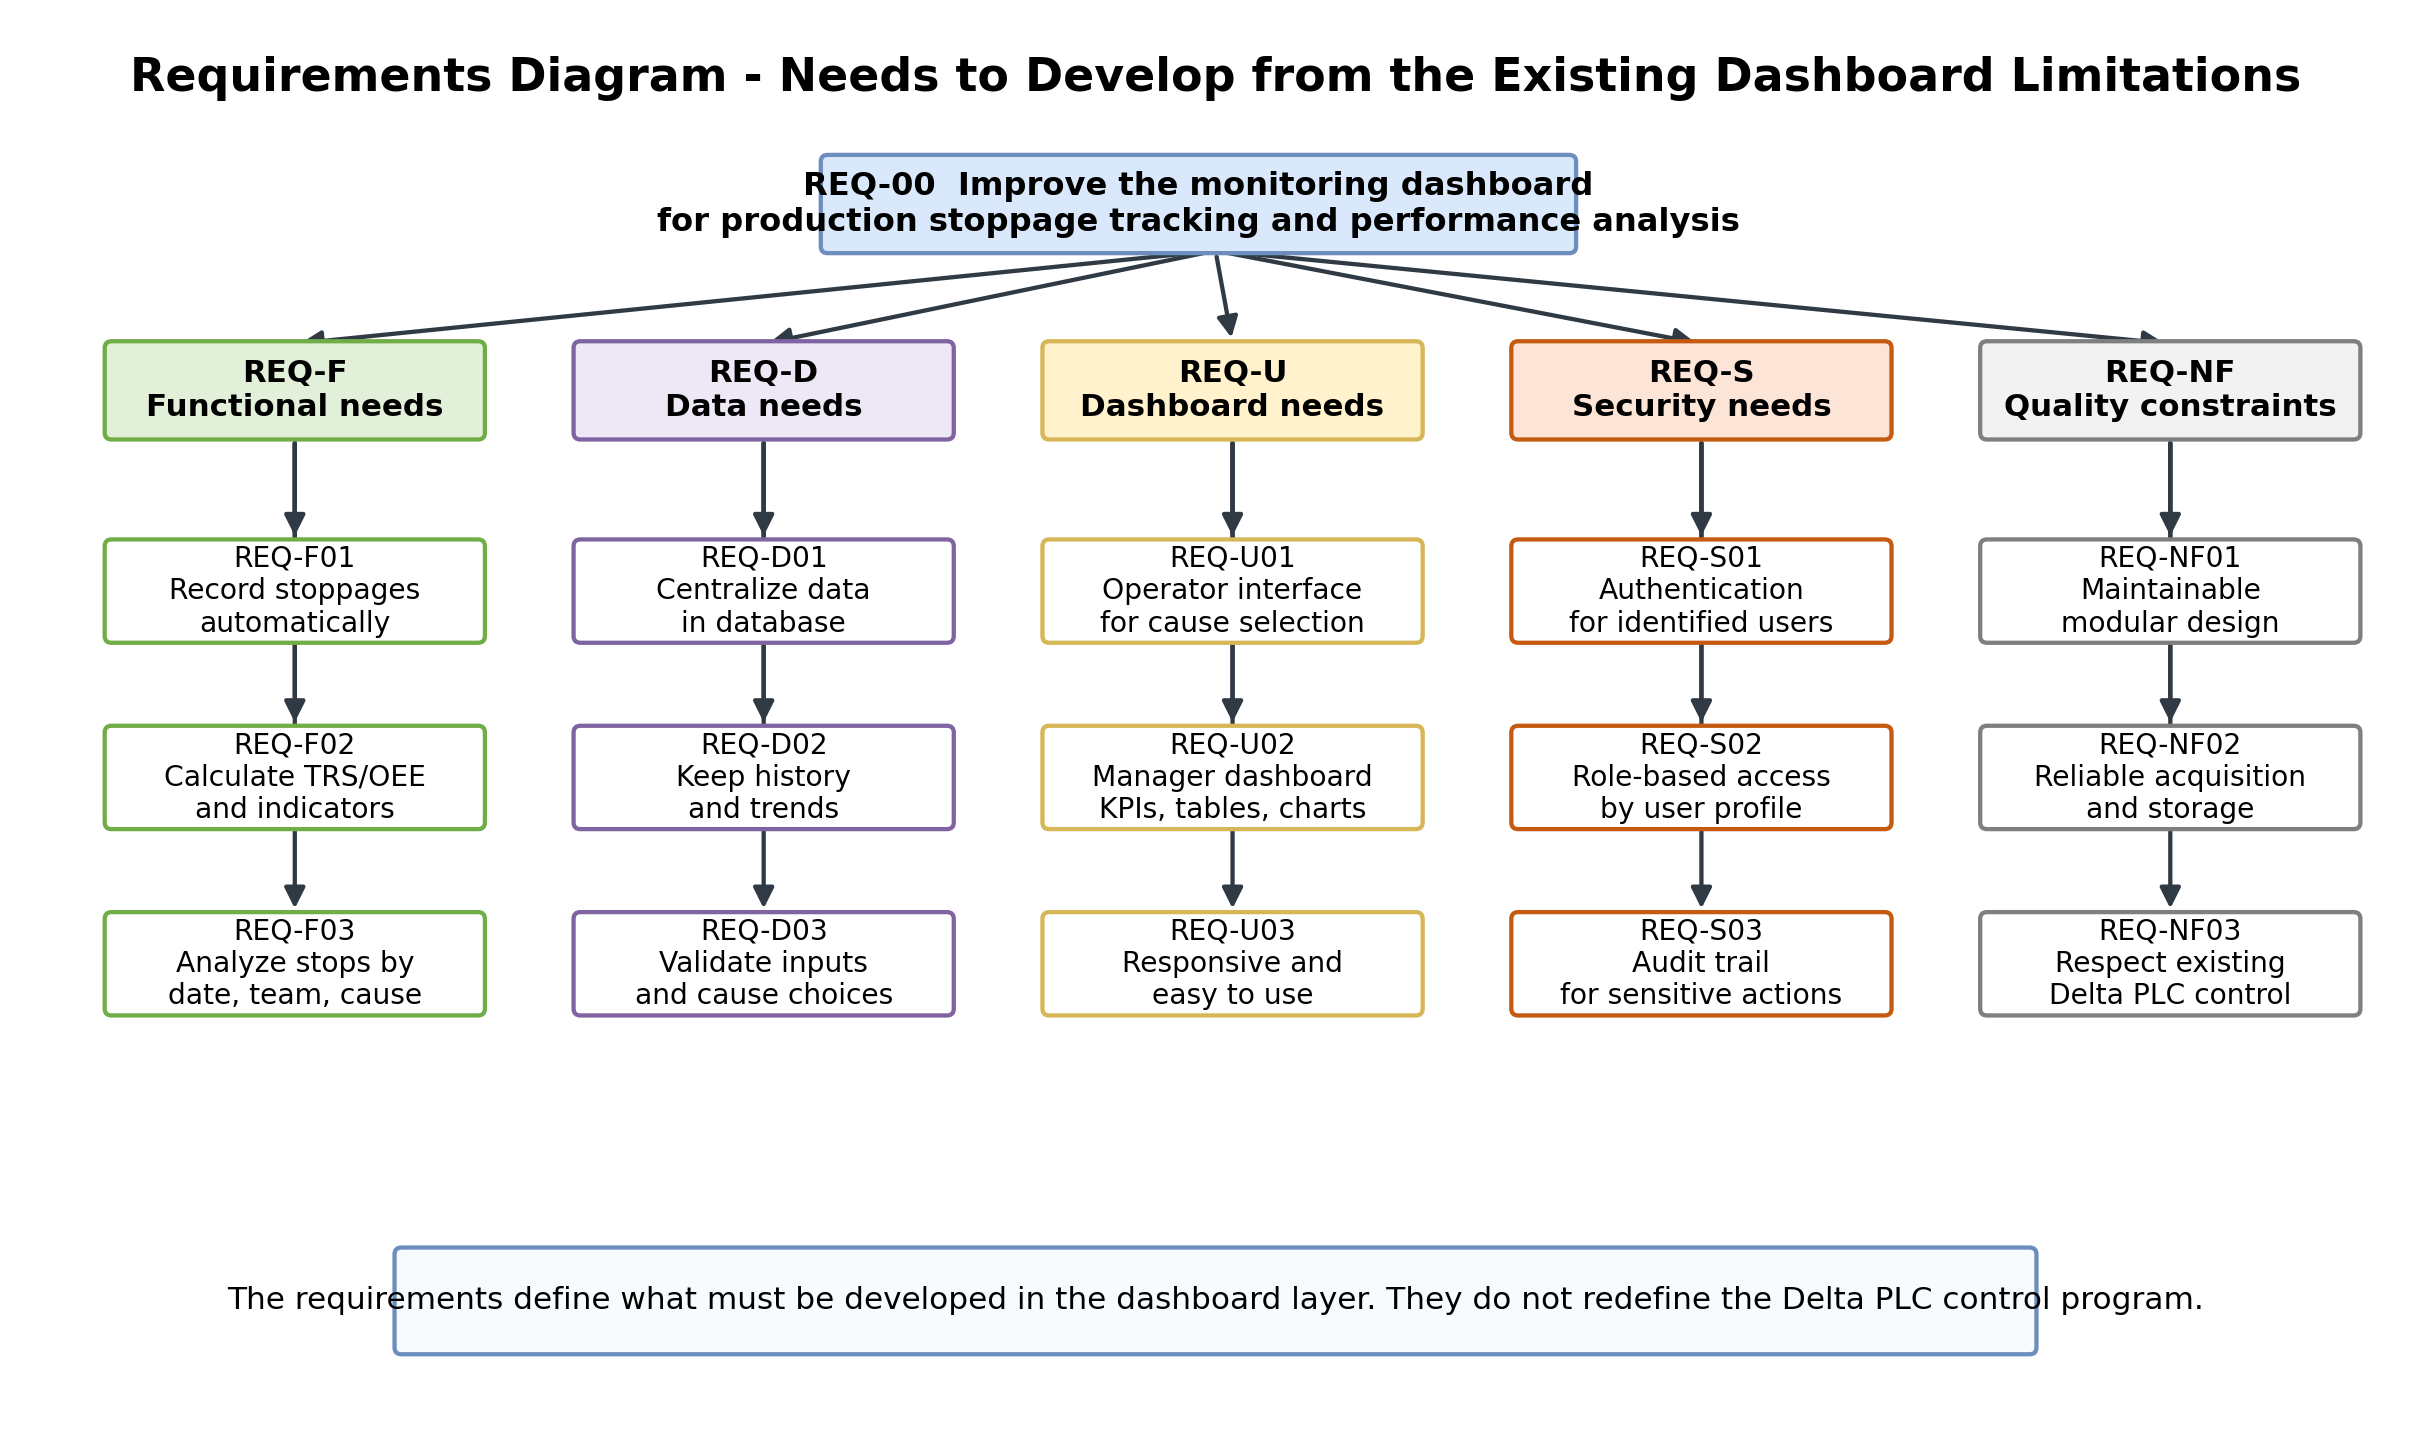
\includegraphics[width=0.9\textwidth, keepaspectratio]{images/requirements_diagram.png}
\caption{Requirements Diagram}
\label{fig:chapter1-5}
\end{figure}

\subsubsection{\fontsize{13}{16}\selectfont Functional Requirements}

\begin{table}[H]
\centering
\caption{Functional requirements of the dashboard to be developed}
\begin{tabular}{|l|l|p{5.5cm}|}
\hline
\textbf{ID} & \textbf{Requirement} & \textbf{Description} \\
\hline
REQ-F01 & Record stoppage events & The dashboard shall record the start time, end time and duration of each production stoppage. \\
\hline
REQ-F02 & Qualify stoppage causes & The operator shall be able to select a stoppage cause from a controlled list of causes. \\
\hline
REQ-F03 & Calculate indicators & The dashboard shall calculate TRS/OEE, total downtime, total productive time and number of stoppages. \\
\hline
REQ-F04 & Display real-time information & The dashboard shall display the latest machine and production information without relying only on manual consultation. \\
\hline
REQ-F05 & Analyze stoppage history & The manager shall be able to analyze stoppages by date, team, cause and duration. \\
\hline
REQ-F06 & Compare periods and teams & The dashboard shall allow comparison between days, shifts or teams to identify recurring performance issues. \\
\hline
REQ-F07 & Manage stoppage causes & Authorized users shall be able to add, modify, disable or delete stoppage causes. \\
\hline
REQ-F08 & Generate reports and exports & The dashboard shall allow the export of production data and indicators for reporting and further analysis. \\
\hline
\end{tabular}
\label{tab:chapter1-1}
\end{table}

\subsubsection{\fontsize{13}{16}\selectfont Non-functional Requirements}

\begin{table}[H]
\centering
\caption{Non-functional requirements and industrial constraints}
\begin{tabular}{|l|l|p{5.5cm}|}
\hline
\textbf{ID} & \textbf{Requirement} & \textbf{Description} \\
\hline
REQ-NF01 & Maintainability & The future dashboard shall be organized so that business logic, interface logic and data access can be maintained clearly. \\
\hline
REQ-NF02 & Scalability & The system shall support future extension of indicators, users and data volume. \\
\hline
REQ-NF03 & Reliability & Data acquisition, storage and visualization shall be stable enough for production monitoring. \\
\hline
REQ-NF04 & Performance & Dashboard pages and filters shall respond quickly enough for daily production follow-up. \\
\hline
REQ-C01 & Preserve PLC control & The dashboard shall not disturb the validated control logic executed by the Delta PLC. \\
\hline
REQ-C02 & Respect existing data sources & The system shall be designed according to the existing industrial data context: Delta PLC, Node-RED flows and MySQL data. \\
\hline
REQ-C03 & Minimize operator burden & The dashboard shall not add unnecessary steps to the operator workflow. \\
\hline
\end{tabular}
\label{tab:chapter1-2}
\end{table}

\section{\fontsize{15}{18}\selectfont Modeling languages: SysMl}

SysMl, or Systems Modeling Language, is a graphical language used by MBSE (Model-Based Systems Engineering) practitioners to create system models and communicate ideas about system designs to stakeholders. It is a language that has a grammar and vocabulary consisting of graphical notations that have specific meanings. The purpose of SysML is to visualize and communicate a system's design among stakeholders \cite{sysml_modeling}.

The grammar and notations of SysML are defined in a standards specification published by the Object Management Group, which is a consortium of computer industry companies, government agencies and academic institutions. SysMl is an extension of a subset of the Unified Modeling Language (UML), and its complete definition requires referral to parts of the UML specification document as well \cite{sysml_modeling}.

We can name a few types of SysMl diagrams:

\begin{itemize}
    \item \textbf{Behavior diagrams \cite{sysml_modeling}}
    \begin{itemize}
        \item Activity diagram
        \item State machine diagram
        \item Sequence diagram
        \item Use case diagram
        \item Communication diagram
    \end{itemize}

    \item \textbf{Structure diagrams \cite{sysml_modeling}}
    \begin{itemize}
        \item Block definition diagram
        \item Internal block diagram
        \item Parametric diagram
        \item Package diagram
        \item Composite structure diagram
    \end{itemize}

    \item \textbf{Requirement diagram[5]}
\end{itemize}

\section*{\fontsize{15}{18}\selectfont Conclusion}

\hspace*{\parindent}Overall, chapter 1 has provided the necessary foundation for the subsequent chapters, enabling a
comprehensive exploration of the problem and the development of an effective solution. By understanding the host company, the specific problem through the case study and the modeling language
employed, you the reader will be equipped with the context and knowledge required to delve deeper
into the next chapters presented in this report.